\documentclass[a4paper, 12pt, final]{hitec}
\usepackage[T1]{fontenc} % this makes text underscore look better
\usepackage{textcomp} % load symbol definitions
\usepackage{underscore} % allows the use of _ in text without escaping
\usepackage[english]{babel}
\usepackage[english]{isodate}
\usepackage[parfill]{parskip}
\usepackage{ragged2e}
\usepackage{appendix}
%\usepackage[none]{hyphenat}% enable to switch off hypenation
\usepackage{times}
\usepackage{setspace}
\usepackage{enumitem}% http://ctan.org/pkg/enumitem
\usepackage{tabulary}
\usepackage{longtable}
\usepackage{inputenc}
\usepackage{amssymb}
\usepackage{amsfonts}
\usepackage[pdftex]{graphicx}
\usepackage[dvipsnames]{xcolor}
\usepackage{subcaption}
\usepackage{wrapfig}
\usepackage{float}
\usepackage{fancyvrb}

% package animate is used for animating PNGs to mimic animated GIFs
% the following command should be used to prepare PNGs from animated GIFs:
% gifsicle --unoptimize animated.gif | convert - frame-%d.png
\usepackage{animate}

\usepackage{alltt}
\usepackage{moreverb}
\usepackage[singlelinecheck=false, justification=centering]{caption}
\usepackage{booktabs,array}
\newcolumntype{?}{!{\vrule width 1pt}}
\makeatletter
\def\thickhline{%
  \noalign{\ifnum0=`}\fi\hrule \@height \thickarrayrulewidth \futurelet
   \reserved@a\@xthickhline}
\def\@xthickhline{\ifx\reserved@a\thickhline
               \vskip\doublerulesep
               \vskip-\thickarrayrulewidth
             \fi
      \ifnum0=`{\fi}}
\makeatother

\newlength{\thickarrayrulewidth}
\setlength{\thickarrayrulewidth}{2\arrayrulewidth}
% for more info on hyperref package see http://en.wikibooks.org/wiki/LaTeX/Packages/Hyperref
\usepackage[pdftex,colorlinks=true,linkcolor=BlueViolet]{hyperref}

\addto{\captionsenglish}{\renewcommand{\abstractname}{Executive Summary}}

\usepackage{lastpage}

\renewcommand{\baselinestretch}{1.1}

%% important to have floats such as tables stick to the top if option [t!] is used
\makeatletter
\setlength{\@fptop}{0pt}
\makeatother

\let\footruleskip\undefined
\usepackage{fancyhdr}

\addto\captionsenglish{% Replace "english" with the language you use
  \renewcommand{\contentsname}%
    {Table of Contents}%
}

\title{Layered Architecture Overview}
\author{Your Company}
\date{\today}
\usepackage{hyperxmp}
\hypersetup{
    pdftitle={User Manual: how to use you system},
    pdfauthor={Your Company},
    pdfsubject={Once sentence description on the manual.},
    pdfcopyright={Copyright (C) 2019 by Your Company.  All rights reserved.}
}

\makeatletter
\let\thetitle\@title
\let\theauthor\@author
\let\thedate\@date
\makeatother

\pagestyle{fancy}
\fancyhf{}
%\rhead{\theauthor}
\lhead{\thetitle}
\cfoot{\thepage}


\captionsetup[table]{font=footnotesize, labelfont=bf}
\captionsetup[figure]{font=footnotesize, labelfont=bf}
\captionsetup[subfigure]{font=scriptsize, labelfont=bf}

%----------------------------------------------------------------------------------------
%	DOCUMENT MARGINS
%----------------------------------------------------------------------------------------

%\textwidth 6.75in
\textheight 25cm
%\oddsidemargin -.25in
%\evensidemargin -.25in
\topmargin -1cm
%\longindentation 0.50\textwidth
%\parindent 0.2in



%----------------------------------------------------------------------------------------
%	TIKZ magic
%----------------------------------------------------------------------------------------

\usepackage{tikz}
\usetikzlibrary{shadows}

\newcommand*\keystroke[1]{%
  \tikz[baseline=(key.base)]
    \node[%
      draw,
      fill=white,
      drop shadow={shadow xshift=0.25ex,shadow yshift=-0.25ex,fill=black,opacity=0.75},
      rectangle,
      rounded corners=2pt,
      inner sep=1pt,
      line width=0.5pt,
      font=\scriptsize\sffamily,
      minimum width=1.2em
    ](key) {#1\strut};
}

%----------------------------------------------------------------------------------------
%	DOCUMENT CONTENT
%----------------------------------------------------------------------------------------

\begin{document}
	\onehalfspacing
	\pagenumbering{roman}
    \begin{titlepage}

	\centering
    \vspace*{0.5 cm}
	\rule{\linewidth}{0.2 mm} \\[0.4cm]
	\begin{spacing}{1.1}
		\huge \bfseries Layered Architecture\\[0.3cm]
		\LARGE Problematic And Overview of Famous Solution by Sashko Potapov
	\end{spacing}
	\rule{\linewidth}{0.2 mm} \\[1 cm]


	\textsc{\large $Document Version$ 1.0.0}\\[4cm]

	% uncomment the following block to add a logo
	% \begin{center}
	% \includegraphics[height=4cm]{sections/00-toc/images/logo.pdf}
	% \end{center}

 
	\vfill
	\noindent
	\begin{minipage}{0.7\textwidth}
		\begin{flushright}
			\textsc{Project:}\\
			\textsc{Draft Date:}\\
		\end{flushright}
	\end{minipage}~~\hspace*{1 cm}
	\begin{minipage}{0.3\textwidth}
		\begin{flushleft}
			1.0.0\\
			01.11.2020\\
		\end{flushleft}
	\end{minipage}

	\clearpage

	\setcounter{page}{1}
	\justifying
	In this essay I briefly give an overview of layered architecture and share my thoughts on this in practical application with an iOS development.
    \clearpage
	
    \setcounter{tocdepth}{3}
    \tableofcontents

    \clearpage

\end{titlepage}

    \pagenumbering{arabic}
    \section{Layered architecture and smart UI overview}\label{sec:01}
    Layered architecture is a great concept, well described in the book «Domain Driven Design» by Eric Evans. This is a very good concept for separation of concerns. In this essay I would like to share my thoughts on this approach from my experience as an iOS software engineer. So Eric Evans describes four layers of a software solution: UI, Application layer, Domain layer and Infrastructure layer. Each of this layers has its own purpose and responsibility, which helps us not only to separate concerns, but to easily change some parts of a software(chage database, because it is connected via interface etc.) and reuse existing(use iOS`s Application, Domain and Infrastructure layers to connect to MacOS`s, WatchOS, tvOS UI etc.). But as Eric Evans  describes some great advantages and disadvantages of it, which I mostly agree, might be a stopper some teams. The most important disadvantage, in my opinion, is it is very difficult to work with layered architecture for a team of inexperienced developers and we have to spend some time digging deep into this topic in order to make software development process smooth and easy. 

	And what about smart UI? Actually Eric Evans explained a really good point, and even better to say mindset of any developer who is willing to implement this pattern. «Put all business logic into the user interface. hop the application into small functions and implement them as a separate user interfaces, embedding the business rules into them. Use a relational database as a shared repository of data. Use the most automated UI building and visual tools available». And this is exactly one of the most common problems with modern MVC implementation. In the next chapter I would like to explain why Apple`s MVC is a smart UI, and what problems  and confusions regular developers face trying to separate concerns simply using MVC in iOS applications.
\section{Overview of Apple`s MVC architecture in iOS}\label{sec:02}
When you start developing iOS applications, first tutorials that you will see will belong to Apple. You read all their fancy documentation, gets excited with Swift`s syntax sugar and finally start building you first app. On their website( https://developer.apple.com/library/archive/documentation/General/Conceptual/DevPedia-CocoaCore/MVC.html ) they suggest to you to use MVC, describing the responsibility of every module and connection between them.
	\begin{figure}[!htbp]
	\centering
	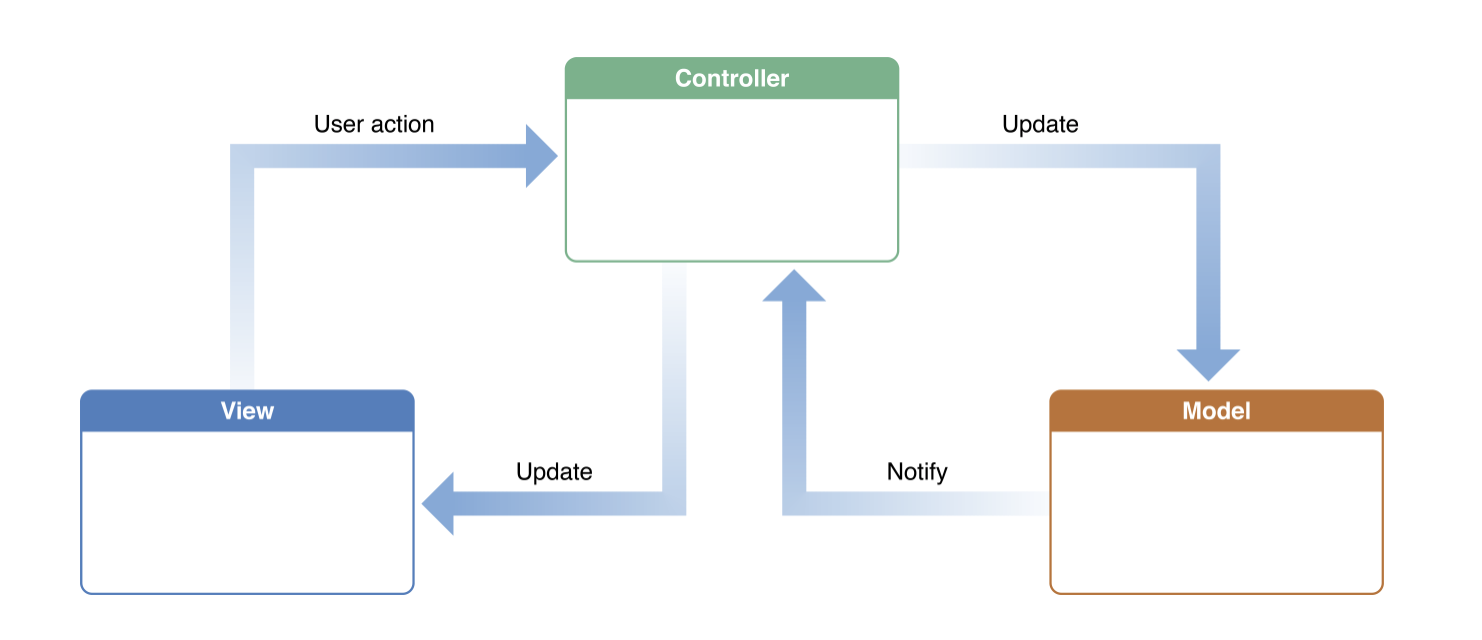
\includegraphics[width=0.95\linewidth]{sections/01-chapter/images/Controller.png}
	\caption{MVC on Apple Website.}\label{sec:01_01:fig:01}
	\end{figure}
But the main problems appears when you are trying to implement it in your first app. But first I have to describe the peculiarity of iOS development. There are two approaches of building the UI layer available today: imperative and declarative. There are no problems with declarative approach, it is available using newly presented ui framework called SwiftUI, it forbids for developers to include any business logic into UI layer by design, but is is available for developer for a year now. This framework is on early stage of beta-testing, so it is not really useful for real-life development. But we are going to look at the most popular framework, which imperative called UIKit. To prove its popularity lets check the reversed-engineered code of the latest iOS 14 https://apptractor.ru/info/articles/kakie-jazyki-programmirovanija-ispolzujutsja-vnutri-ios-14.html and SwiftUI is less than 1 percent of overall code. So with UIKit there are two main approaches of building UI - visually via XML file and from code via Swift. Apple provides us with starting base class called UIViewController, which is responsible for holding UI object with strong reference and process user gestures and actions(swipes, button touches etc.). Junior developers love to build UI from XML, sometimes is very useful and very easy to understand for new developers, because they do not have to read UI from code and imagine how it looks like on device.  So we are going to see how this approach works. You have your UI built in XML file and some its views connected to UIViewController class using @IBOutlet and @IBActions decorators. And your UIViewController class is not fully a view, since you have your view built in xml, and fully a controller, because it has some UI views and user actions connected. At this point your UIViewController becomes smart UI, where you handle user gestures, change UI and store business logic. Furthermore, iOS SDK gives you very useful decorators to easily use persistence storage - SQLite Database. So not only UIViewController combines UI layer, Domain layer and Infrastructure layer, but also handles navigation logic, dependency injection etc., so responsibility of Application layer is also on UIViewController. There is a huge temptation to use smart UI like this for small projects, but very often your UIViewController exceeds 800 lines, than 1000 lines, and at some project I have seen 5000 lines UIViewController. 


    \section{Examples from iOS development using Swift}\label{sec:03}

In previous chapter we described the problematic of MVC approach in Apple`s example. So there is a question: «How to use proper layered architecture in an iOS app, what its advantages and disadvantages will be?». The community came with an idea of using MVVM architecture aka proper MVC. Model-View-ViewModel is a response for inappropriate MVC, which came as a resue because of impossibility to test business logic of an application. So the main point is to separate any UI with business logic. We have a dummy view in UIViewController aka UI layer aka View, business logic in ViewModel aka Domain layer and Networking/Persistence/Other managers in Model aka Infrastructure layer. Still we are missing Application layer, so this responsibility might be taken by UIViewController, but we do not want this for sure and Coordinator pattern comes to rescue. Coordinator pattern separates UI layer from Application layer. In the end we have such modules connection.
\begin{figure}[!htbp]
	\centering
	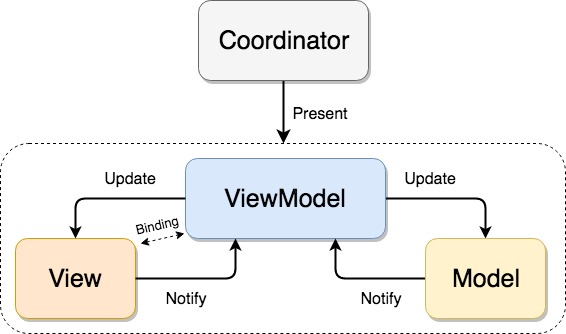
\includegraphics[width=0.95\linewidth]{sections/02-chapter/images/Coordinator.jpg}
	\caption{MVVM-C architecture.}\label{sec:02_01:fig:02}
	\end{figure}
    
Imagine that you are simply separating those concerns you can not only copy-paste Domain layer, Application layer and Model layer code from iOS to MacOS/WatchOS/tvOS app(only rewriting UI layer) but also Unit-tests which you used to cover you ViewModel. Bingo!!! Everything looks super-great, well in theory it is. But in practice we stuck in some serious issues, mostly related to data binding. What is data binding? Well, imagine that you have a two classes which are connected via composition. In our example it is UIViewController has a property called ViewModel. How to make UI respond to changes in ViewModel? How to make ViewModel react to changes in persistence storage? How to make ViewModel react to changes on server(let`s imagine we have a hook)? How to make UI react to changes in database? So communication between so many layers becomes a serious issue. We have a lot of solutions: callback via closures aka lambda function, delegates, some reactive binding etc. While MacOS sdk provides native data binding called Cocoa-bindings we do not have any useful instrument in iOS SDK and have to use callback, specifying that it have to be called on main thread each time etc. But community comes to rescue ti Rx frameworks (RxSwift and RxCococoa) and huge amount of useful reactive extensions. Those frameworks are universal for all Apple platforms, which makes them very useful and extremilly popular. Everything looks super-great but for one thing. Reactive programming is another  galaxy in development, which is so far from Junior developers that you should forget the idea of making cool reactive app with team who has those guys in it. Those frameworks requires changing a mindset from object-oriented programming to reactive functional programming which is not so easy. We can not use any reactive framework for sure and simply live with native solutions which we have from the box - callbacks and delegates, those patterns much easier to understand and use but they requires a lot of code, which slows down the development process and sometimes becomes very confusing to have dozens of objects which a delegates to other dozens of objects. I guess a team-leader should pick the most suitable solution for the particular team and particular project needs. Maybe MVC-C will become a great solution in terms of complexity/speed, maybe MVVM-C with delegates is a good one or even classic MVC is enough for project with no possibility of user action(for ex. currency exchange app which only provides info).

\end{document}

